\documentclass[a4paper,11pt]{jarticle}

\setlength{\oddsidemargin}{0pt}
\setlength{\textwidth}{450pt}
\setlength{\topmargin}{0pt}
%%%%%%%%%%%%%%%%%%%%%%%%%%
%%%%%上
\setlength{\topmargin}{-1.0mm}% 25.4mm-25.4mm
\setlength{\headheight}{8.mm}%
\setlength{\headsep}{2.mm}%
%%%%%本文縦
\setlength{\textheight}{230mm}%
\setlength{\footskip}{15mm}%
%%%%%左
\setlength{\oddsidemargin}{0mm}% 25.4mm-25.4mm=0mm
\setlength{\evensidemargin}{0mm}%
%%%%%本文横
\setlength{\textwidth}{159.2mm}%
\usepackage{fancyhdr}
\usepackage{here}
\usepackage{graphicx}
\usepackage{enumerate}
\usepackage{amsmath}
\pagestyle{fancyplain}
\lhead{\small A group 研究会資料}
\rhead{\small 2001/10/23(Tue.)}


%%%%%%    TEXT START    %%%%%%
\begin{document}
%	\baselineskip = 0pt
	\begin{center}
		{\Large {\bfseries カメラ画像の色分け閾値の自動生成および実時間更新}}
	\end{center}
	\begin{flushright}
		RoboCupグループ  M1  上田 隆一  \\2001/10/23
	\end{flushright}

\section{序論}
%色の情報は, カラーカメラが搭載されたロボットにおいて重要な情報となる. 
特に人工ランドマークなど, 人間があらかじめ色を決定できるものに対しては,
閾値処理でその色を抽出する方法が直感的で分かりやすい. 
しかし, 閾値処理においては, 照明条件の変化が, しばしば問題となる. 
また, 閾値の設定方法が経験的であることや, 時間がかかって面倒であることも,
問題である. 


RoboCup Legged Robot Leagueでは, フィールドやその周辺の物体は,
人間には容易に識別できる色で塗り分けされているにもかかわらず
(図\ref{fig:field},表\ref{tab:collabel}), 電球が劣化したり,
自然光が窓から差し込んだりするだけで, ロボットの判断力に影響が出る. 
電球の劣化は連続的であるため, RoboCupチームがロボットを使って実験する際には,
事前に閾値 (AIBOに関わる人々は, カラーテーブルと呼んでいる) 
の調節を行わなければならない. 
また, 各ロボットのCMOSカメラには個体差があり,
ロボットごとにカラーテーブルの調節を行う必要があることも,
面倒さに拍車をかけている. 


\begin{figure}[h]
	\begin{center}
	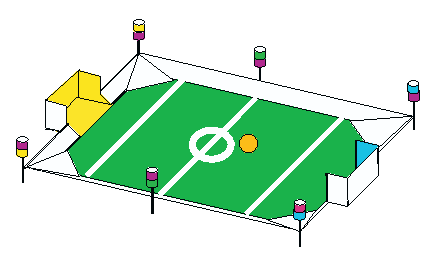
\includegraphics[width=0.8\linewidth]{Fig/field.eps}
	\caption{フィールド}
	\label{fig:field}
	\end{center}
\end{figure}[h]
\begin{table}[h]
\begin{center}
\begin{small}
\caption{色分け}\label{tab:collabel}
\begin{tabular}{l|l}
\textbf{物体} & \textbf{色} \\
\hline
ボール	& オレンジ\\
ゴール	& スカイブルー, 黄\\
ランドマーク	& ピンク, スカイブルー, 黄, 緑\\
フィールド	& 濃緑\\
他機のユニフォーム	& 赤, 青\\
壁	& 白
\end{tabular}
\end{small}
\end{center}
\end{table}

そこで本研究のテーマを, 色分けのための閾値を自動生成するアルゴリズムと,
閾値を照明条件の変化に対して動的に変化させるアルゴリズムの実装とする. 
具体的には, 以下のようなアルゴリズムをAIBOに搭載することを目標とする. 


\begin{itemize}
	\item カラーテーブルの自動生成\\
事前知識なしで, カメラの画像から特徴のある単色を検出し,
カラーテーブルに記憶する. 

	\item カラーテーブルの実時間更新\\
事前に用意されているカラーテーブルを,
照明条件の変化に対応して実時間で調節する. 

\end{itemize}
本稿では, 前者の従来法, 課題, 進捗状況について述べる. 


\section{従来のカラーテーブル作成法と課題}
Legged Robot Leagueで問題となることに,
カラーテーブルの形式が実際の色の分布と合わないことが挙げられる. 
カラーテーブルは, AIBOに搭載されたハードウェアが使用するため,
このハードを使用する限り, フォーマットを変えることはできない. 
デフォルトのカラーテーブルは,
ある色についてYUV空間を次のように切り分ける (図\ref{fig:hard}) . 

\begin{itemize}
	\item Y (輝度) 値を8段階に分割する. 
	\item 各段階において, 1辺がU軸に平行な長方形で,
その色の領域を切り分ける. 

\end{itemize}
しかし, フィールド上でAIBOが撮影した画像の各画素について,
YUV空間での分布状況を見ると, どの色もUV平面状で楕円状に分布しており,
長方形で切り分けようとすると, 隣の色の一部を拾ってしまうことがしばしばある. 

\begin{figure}[H]
	\begin{center}
	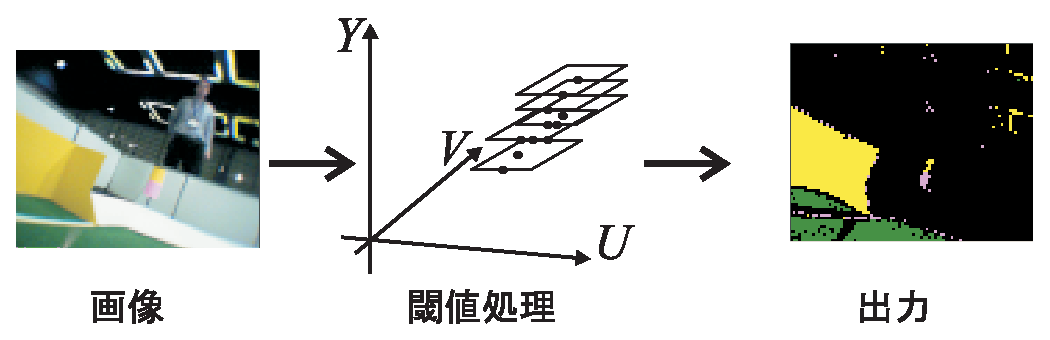
\includegraphics[width=0.99\linewidth]{Fig/hard.eps}
	\caption{AIBOのハードウェア処理}
	\label{fig:hard}
	\end{center}
\end{figure}
去年度のUNSWや, それを真似した今年の九州チームは,
その問題を解決するために, ハードの使用をやめ,
自分たちでカラーテーブルを作成した. 
この方法は, YUV空間を表す3次元配列を使用し,
各セルにはそのYUV値がどの色であるのかを記述しておく. 
そして, カメラが出力する各画素のYUV値
(それぞれ0から255までの値をとる)と比較して, 色を求める. 
この方法は, RoboCupのように整備された環境では非常に有効であり,
デフォルトのカラーテーブルよりも照明条件の変化に強い. 
しかしそれは, 空間の区切り方をデフォルトのカラーテーブルよりも
細かくしただけの話であり,
デフォルトのものとの本質的な違いや斬新さは皆無である. 
また, 配列に色情報を書き込むのが人間の作業であることも,
他の多くのチームと違ってはいない(ただし,
本年度のUNSWチームは異なった方法を採用したかもしれないので,
調査の必要がある). 


カラーテーブルの自動生成は, 昨年度まで当チームで行われてきた. 
このときの自動生成アルゴリズムで一番の問題となったのは,
計算量の多さであった. 
試合会場に行き, カラーテーブルを作成するまでには,
どんなに順調であっても最低3,4時間はかかった. 
現在は, 手動でカラーテーブルを作成しているが,
これはロボット一台あたり
\footnote{最近ロボットのカメラに個体差があることが判明し,
現在はロボット一台ごとにカラーテーブルを作成している. 
}30分で終了するので,
PCよりも人間の方が早くカラーテーブルを作成できるというのが現状である. 
本研究では, 自動生成アルゴリズムを実機に搭載することを目標としているので,
計算量の削減は必須事項である. 


また, 昨年度アルゴリズムは,
画像上のゴールやランドマークの位置を人間が指定する必要があったので,
半手動であった. 
本研究では, 完全な自動生成を目指すこととする. 
そのためには, 環境中の観測対象物の色を学習するアルゴリズムが必要となる. 


\section{自己組織化マップを用いたカラーテーブルの作成}
どのような手法がカラーテーブルの自動生成に有用であるかは現在調査中であるが,
有力なものの一つとして,
ファジー推論ニューラルネットワーク(FINN)\cite{iyatomi}が挙げられる. 
\cite{iyatomi}では, 風景画像から自動的に言語形式
(例:「雲は, 上の方にあり, 明るくにぶい青系統の色です. 
」)による知識の抽出を行い, 画像中の領域の認識を行っているが,
これをそのまま色分けの能力の獲得に利用できそうである. 
(あるいはゴールやランドマークの直接的な識別ができるかもしれない. )

FINNの内部では, 自己組織化マップ (SOM) \cite{kohonen,usui}が用いられている. 
今回はSOM単体でカラーテーブル作成が可能であるか検証する目的と, 
SOMに筆者が慣れる目的を兼ねて, SOMを用いたカラーテーブル作成ツールを試作した. 
以下では, SOMと作成したツールについて説明する. 


\subsection{自己組織化マップ (SOM)}
SOMは, 競合型ニューラルネットワークの一種であり, 
ニューロンは1次元ないし2次元的なつながりを持って配置される. 
各ニューロンは結合重みベクトル
$\boldsymbol{w}_i = (w_{i1},w_{i2},\ldots ,w_{in})$を持つ. 
SOMに, 入力データベクトル
$\boldsymbol{x}_j = (x_{j1},x_{j2},\ldots ,x_{jn})$が投入されると,
各ニューロンは次式により内部ポテンシャル$\text{net}_i^j$を計算する. 

\begin{eqnarray}
\text{net}_i^j = \dfrac{1}{D(\boldsymbol{w}_i - \boldsymbol{x}_j)}
\end{eqnarray}
ここで, $D$は, 
入力データとニューロンの結合重みベクトルの相違度を測る距離関数で,
通常ユークリッド距離
$D(\boldsymbol{w}_i - \boldsymbol{x}_j) = |\boldsymbol{w}_i - \boldsymbol{x}_j|$が用いられる. 


各ニューロンの内部ポテンシャル$\text{net}_i^j \ (i=1,2,\ldots ,n)$
が求まると, 次に, 最大の内部ポテンシャルを示したニューロン$k$を見つける. 
これは, 入力データ$\boldsymbol{x}_j$
に最も類似した結合重みを持つニューロンを探し出すことを意味する. 
そして, ニューロン$k$
とその近傍のニューロンについて以下のように結合重みベクトル
$\boldsymbol{w}_i$を更新する. 

\begin{eqnarray}
\boldsymbol{w}_i(t+1) = \boldsymbol{w}_i(t) + \alpha(t)(\boldsymbol{x}_i - \boldsymbol{w}_i)
\end{eqnarray}
$\alpha(t)$は学習係数であり, 最初0.8くらいにしておき, 次第に小さくする. 
また, 近傍領域の大きさも次第に減少させる. 
このようにして作成されたマップは, 1次元あるいは2次元空間で,
多次元空間におけるデータ相互の距離関係を表現する. 


\subsection{カラーテーブルへのSOMの応用}
SOMにサンプル画像中のYUV値の分布状況を学習させた. 
$n=3$として, $w_{i1},w_{i2},w_{i3}$をそれぞれY値, U値, V値とした. 
図\ref{fig:3d}は, 40枚の画像(88$\times$72画素)
の全pixelを入力した結果である. 
計算時間は, Celeron 600MHzで21秒であった. 
図\ref{fig:3d}のマップを平面に戻して,
各ニューロンの色を表示したものが図\ref{fig:2d}である
\footnote{白黒ですいません. }. 
図\ref{fig:2d}のマップを更に数色に分類することで,
3次元に分布したデータを数色に分類する問題よりも簡単になる. 


上記のアルゴリズムと,
2次元のマップの自動分類アルゴリズムをロボットに実装すれば,
カラーテーブルの自動生成アルゴリズムは完成するが,
今回は後者のアルゴリズムの作成に間に合わなかったので,
図\ref{fig:color}
のようなSOMから手動でカラーテーブルを作成するツールを作成した. 

\begin{minipage}{21em}
\begin{figure}[H]
	\begin{center}
	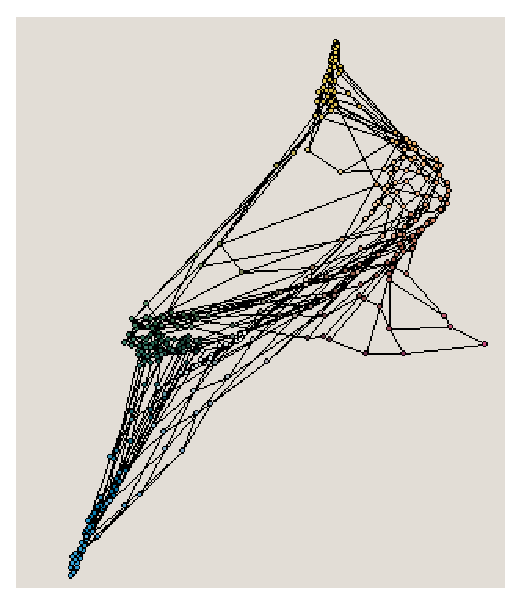
\includegraphics[width=0.8\linewidth]{Fig/3dsom.eps}
	\caption{学習結果(3次元形状)}
	\label{fig:3d}
	\end{center}
\end{figure}
\end{minipage}
\begin{minipage}{21em}
\begin{figure}[H]
	\begin{center}
	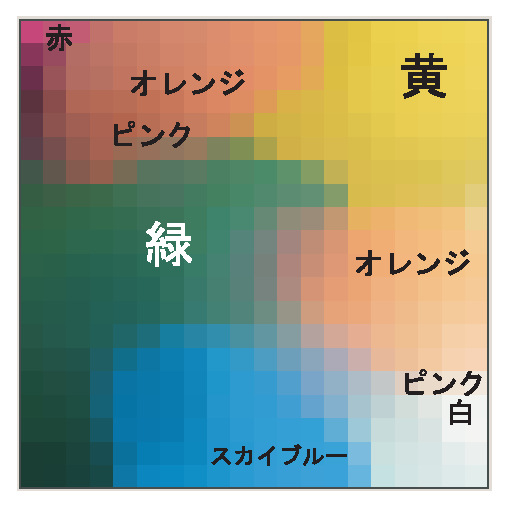
\includegraphics[width=0.99\linewidth]{Fig/2dsom.eps}
	\caption{学習結果(図\ref{fig:3d}を2次元に広げたもの)}
	\label{fig:2d}
	\end{center}
\end{figure}
\end{minipage}
\begin{figure}[H]
	\begin{center}
	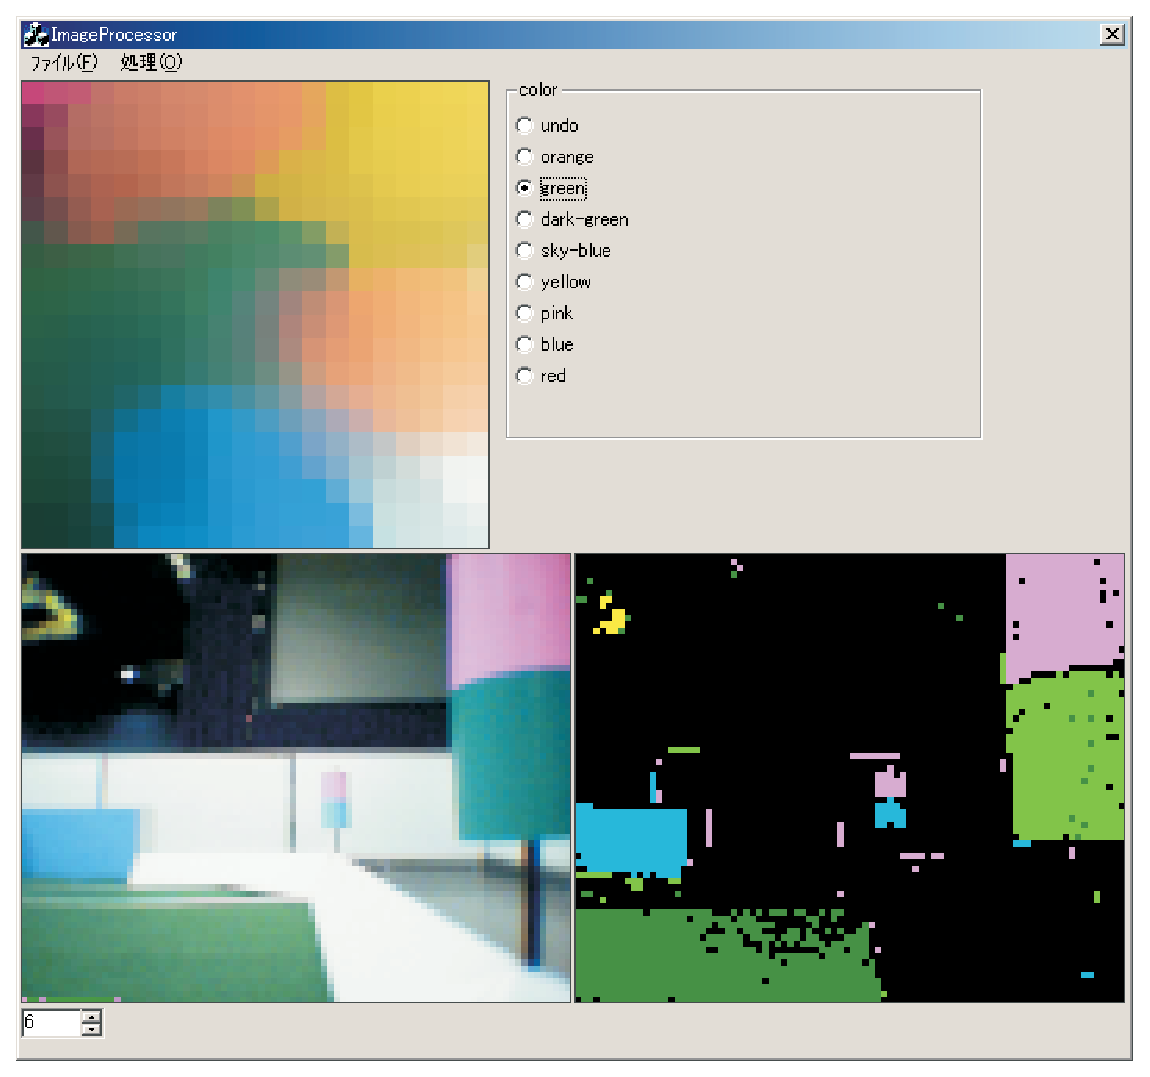
\includegraphics[width=0.7\linewidth]{Fig/color.eps}
	\caption{作成したツール. 
``color''の枠内の色を選択して,
その色と関連付けたいニューロンをクリックすると,
その近傍にあるYUV値がその色に関連付けされ, 左下のように表示される. 
}
	\label{fig:color}
	\end{center}
\end{figure}


\section{考察}
このツールを使用して, 筆者自身で色の関連付けを実行したところ,
SOMを用いることについて次のようなことが判明した. 


\paragraph*{雑音が多い. 
}これは, 雑音と観測対象を全てSOMに入力しているので当然である. 
しかし, たとえ観測したいものだけをSOMに入力しても雑音は取り除けないし,
観測対象と全く同じ色がフィールド外に存在すると,
カラーテーブルで解決できる問題ではなくなる. 
この問題については, AIBOがサッカー中に行う画像処理に,
形状認識アルゴリズムを導入することで対策を取る必要があると考える. 
とは言え, あまり雑音が多いと形状認識アルゴリズムが遅くなってしまうので,
今後, 雑音除去を試みる必要がある. 


\paragraph*{ピンク色の画素が画像中に少ないため, 白色と分離できない. }
手動でカラーテーブルを作成するときは, 白とピンク色は容易に分離できたので, 
ピンク色の画素を重点的に入力すれば解決できる問題ではある. 
しかし, 作成自動化のためには, 
そのような場当たり的な解決法は極力避けるべきであると考えている. 
\\

また, このツールに関しては,
カラーテーブルを作成する人の負担が削減できる可能性があると考えている. 
現状では雑音が多すぎるが, ある程度減らしてやれば,
あとは別のツールで人間が微調整する程度で済むようになる. 
手動でカラーテーブルを作成することは研究テーマではないが,
当面の間チームが使用するものを作成することには意義があるので,
研究と平行して行う必要がある. 


\section{結論と今後の展望}
本稿ではカラーテーブルの自動生成について,
計算量の削減と学習アルゴリズムの実装を課題とし,
自己組織化マップ(SOM)を用いる方法について現在調査中であることを述べた. 
また, 研究途中で作成したツールを用い,
SOMをそのまま用いたときに生ずる問題について説明した. 


今後は, チーム内で色の雑音について,
どれだけカラーテーブルで対処するかの基準を明確にすることと,
色分けを従来通りハードで行うのか,
あるいはソフトで行うのかを話し合う必要がある. 
それらが明確になった後の作業としては,
SOMだけでどこまでできるかを試した後,
FINN等についての導入を検討する予定である. 


\begin{thebibliography}{3}
%\bibitem[野田 1992]{noda} 野田 一雄, 宮岡 悦良:``数理統計学の基礎,''共立出版, 1992. 
\bibitem[臼井 1995]{usui} 臼井 支朗, 岩田 彰, 久間 和生, 淺川 和雄:``基礎と実践ニューラルネットワーク,''コロナ社, 1995. 
\bibitem[Kohonen 1996]{kohonen} Teuvo Kohonen 著 (1996), 徳高 平蔵, 岸田 悟, 藤村 喜久郎 訳:``自己組織化マップ,''シュプリンガー, 1996. 
\bibitem[彌富 1999]{iyatomi} 彌富 仁, 荻原 将文 : ``ファジー推論ニューラルネットワークを用いた風景画像からの知識抽出と認識,''電子情報通信学会論文誌 D-I\hspace{0.1em}I Vol. J82-D-I\hspace{0.1em}I, No. 4, pp.685-693, 1999. 
\end{thebibliography}
\end{document}
